\documentclass[doc]{apa}
\usepackage{url}
\usepackage{verbatim}
\usepackage{moreverb}
\usepackage{graphicx}


%%% make verbatim output smaller
\makeatletter
\def\verbatim@font{\small\ttfamily}
\makeatother
\renewcommand{\tt}{\small\ttfamily}

%\usepackage{hyperref} incompatible with apa
\newcommand{\href}[2]{#2}

\newcommand{\shuffle}{\texttt{shuffle}}

\begin{document}


\title{Shuffle: a program to randomize lists with optional sequential
  constraints}

\acknowledgements{E-mail: \url{pallier@lscp.ehess.fr}. Web: \url{http://www.pallier.org}}


\rightheader{shuffling lists with constraints}

\shorttitle{shuffling lists with constraints}

\author{Christophe Pallier}

\affiliation{INSERM U562, SHFJ, Orsay, France}


\abstract{This paper describes \shuffle, a program to randomize lists of
  items, with the option of setting constraints on successive items. It is
  useful, for example, to extract random samples from a dictionary, or to
  generate quasi-randomized lists of stimuli in which there are no long
  sequences of similar trials. \shuffle{} reads a set of lines and reprints
  them (or a subset of them) in a random order. It is possible to set
  constraints on the output so that no more than a certain number of lines
  with similar labels are repeated, or, on the contrary, so that a minimum
  number of lines separates two lines with the same labels.}

\maketitle

\section*{Introduction}

Experimental psychologists often need to extract random samples and/or to
randomize lists.  For example, psycholinguistics experiments typically
requires extracting random samples of words from dictionaries.  Or, the order
of trials administrated to participants often needs to be randomized.

Presenting the stimuli in different random orders to each participant aims to
diminish the impact of list-specific potential between-trials interactions.
Some between-trials interactions arise when series of trials contains long
sequences with similar characteristics; For example, successive trials may
contain stimuli that have similar features, or map systematically onto the
same response. It is known that response times of participants are sensitive
to such local repetitions \cite{Luce86}.

This paper presents \verb|shuffle|, a program designed to extract
random samples and to `quasi-randomize' the order of items in a list,
avoiding long runs of similar items, or, on the opposite, imlposing a minimum
interval between repetition of given categories of items. 

\section*{Installing shuffle}

The ``shuffle'' package can be freely downloaded from the software page on the
author's web site (\href{http://www.pallier.org}{http://www.pallier.org}). It
consists of two programs: \texttt{shuffle} and \texttt{shuffle.tk}. The first
is meant to be used from a command line, while the other provides a graphical
interface. New users will probably like better the version with the graphical
interface, but the command line version has additional options, no limitation
on the size of the input and embodies the unix philosophy of designing small,
portable and efficient tools that can easily be used as building blocks in
more complex programs. It will therefore appeal more to advanced users.


Both programs are written in Perl
(cf.~\href{http://www.perl.com}{http://www.perl.com}, \cite{randal01}).
Therefore, before using them, an interpreter for the language Perl must be
installed on your computer (cf.~Appendix for instruction for Windows users).
Moreover the Tk module for Perl must be installed to use the graphical version
\cite{walsh99}.  One of the advantages of having shuffle written Perl, is that
it can run under Linux, MacOS-X, Windows...  Another is that one can modify,
if needed, the source code to tune it to ones' requirements.  ``shuffle'' is
distributed under the terms of the GNU General Public License 2 \cite{GPL}.

Once Perl is setup, to install the ``shuffle'' package, you need to:
\begin{enumerate} 
\item copy \texttt{shuffle} and \texttt{shuffle.tk} in a directory listed in
  the PATH variable (e.g.  \texttt{~/bin} under Linux, \texttt{c://windows}
    under Windows.).
  \item adapt, if necessary, the first line of each program, to reflect to
    actual location of perl on your system. The original files assume that the
    perl program is located at \texttt{/usr/bin/perl}. You may have to change
    this to, for example, \texttt{/usr/local/bin/perl} (To locate perl, under
    unix/linux, just type `which perl' on a command line).
\end{enumerate}

\section*{Using `shuffle'}

Typing `\texttt{shuffle.tk}' on a command line launches the graphical version
(see Figure~\ref{tk}.)

\begin{figure}[h]
\begin{center}
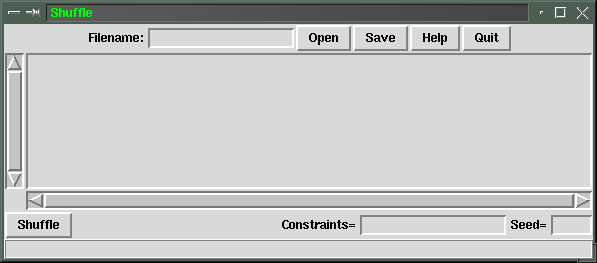
\includegraphics[width=12cm]{shufftk}
\end{center}
\caption{Main window of shuffle.tk}\label{tk}
\end{figure}

The center of the window features a text area where the original list can be
entered, with one item per line. The list can be edited directly or pasted
from the clipboard. Alternatively, it can be read from a text file by typing
first the filename in the box entitled `Filename' and pressing then the `Open'
button.\footnote{The user should be aware that there is a limitation on the
  size of the text that can be put in a text area in a graphical interface.
  This limitation varies from one operating system to the other, so no general
  limit can be given, but we should be cautious when pasting more than, e.g.
  32000 characters. If in doubt, use the command-line version.}

Pressing the `shuffle' button shuffles the lines in the text area in a random
order. The ``seed'' box can be used to enter a number which characterizes the
permutation that will be used. This is useful if one want to apply the same
permutation to several lists.

If the ``constraints'' box is empty, all permutations are allowed and are
equiprobable. To constraint permissible permutations, it is possible to enter
a series of numbers in this box.  This option is meaningful only when the
input text is in tabular format, that is when each line contains the same
number of items separated by spaces. The items in some or all of the columns
may be considered as ``labels'' corresponding to levels of experimental
factors. It is then possible to reject permutations in which the labels are
repeated, across successive lines, more than a fixed number of times. For
example, if a column contains the labels `WORD' or `PSEUDO', one may want to
avoid permutations in which, say, more than four lines in row contain the same
label.

The \textit{$i^{\mbox{th}}$} number in the constraint box corresponds to the
\textit{$i^{\mbox{th}}$} column in the input. When set to '0', there is no
constraint in the relevant column. When set to a positive number, it means
the maximum number of repetitions (across successive lines) in the relevant
column. When set to a negative number, e.g. $-n$, it means that a least $n$
lines must separate two occurrences of the same label.

The latter option is useful, for example, to generate lists where a small
number of targets are interspeded in between a larger number of filler items:
a column could be created containing either the label `TARGET' or 'FILLERxxx'
where `xxx' varies for each filler. If the constraint `-10' is associated to
this columns, targets will be separated by at least 10 fillers.

The command line utility will be described briefly. The examples assume that
the input list is in a text file named `corpus.txt' in the current working
directory. The command:
\begin{verbatim}
shuffle corpus.txt
\end{verbatim}  
prints the lines from \verb|corpus.txt| in a random order. In
order to save this result in a text file, one must use the redirection
operator `\verb|>|': the following command: 
\begin{verbatim}
shuffle corpus.txt >neworder.txt
\end{verbatim}
produces a random permutation of the lines of \verb|corpus.txt| and stores it
in the file \verb|neworder.txt|.

Often, one does not need a complete permutation, but rather only a
random sample from the original list. The variable 'n', passed as
argument to \shuffle{}, permits to specify the maximum number of
output lines:
\begin{verbatim}
shuffle n=10 corpus.txt
\end{verbatim}
yields 10 lines picked at random from \verb|corpus.txt|. The variable
\texttt{seed} can also be set on the command line. This can be useful to apply
the same permutation to different files:
\begin{verbatim}
shuffle seed=123 corpus.txt
shuffle seed=123 corpus2.txt
\end{verbatim}

Finally, to specify constraints on the repetition of labels in columns, one
must pass the variable `constr' on the command line:
\begin{verbatim}
shuffle constr='0 0 4 -6' corpus.txt
\end{verbatim}

Listing~1 shows a few examples of the use of 'shuffle'. Note that in
these examples, 'shuffle' just displays its result. To save it in a
file, one has to use the redirection operator '\verb|>|'.

\begin{figure}[tb]
\caption{Listing~1: a few examples of shuffle's use}
\hrule\vspace*{4pt}
\begin{verbatim}
shuffle -?               # to display a short help
shuffle sample.txt
shuffle n=10 sample.txt  # limits output to 10 lines
shuffle n=10 sample.txt  # new permutation of 10 lines
shuffle n=5 seed=134 sample.txt # sets the seed of the random generator
shuffle n=5 seed=134 sample.txt # you get the same permutation as before...
shuffle n=8 constr='2' sample.txt # no more than 2 succesive lines with
                                  # the same value in column 1
shuffle n=8 constr='0 3' sample.txt # no more than 3 succesive lines with
                                    # the same value in column 2
shuffle n=8 constr='2 2' sample.txt # no more than 2 successive lines with
                                   # the same values in column 1 or column 2
shuffle n=8 constr='1 1' sample.txt # not much room for randomness
\end{verbatim}
\hrule
\end{figure}


\section*{Proof of equiprobability}

Here is the pseudo-code for the generation of an unconstrained random
permutation:

\begin{verbatim}
...read line[1] to line[N]
for i := N downto 2 do swap( line[i], line[random(i)] )
//  remark:  random(i) return a number in the interval [1;i]
\end{verbatim}

We are going to use the recurrence principle to demonstrate that this
algorithm makes all permutations of the lines equiprobable (that is,
each has the probability $1/n!$). It helps to note that the
previous code is the iterative equivalent of the following recursive
algorithm:

\begin{verbatim}
function perm(n) {
 swap(line[n],line[random(n)])
 if n>1 then perm(n-1) 
}
\end{verbatim}

For a permutation of size 2: line[2] is swapped either with line[1] or with
line[2] (itself), each case having probability 1/2. Therefore the two
permutations, (1,2) and (2,1), are equiprobable.
 
Let us suppose that the algorithm generates equiprobable permutations up until
rank $n-1$ (that is, any given line has probability $1/n-1$ to occur in any
given output rank). To generate a permutation of rank $n$, the algorithm first
swaps line[n] randomly with one of the lines between 1 and $n$ (therefore each
has the same probability, $1/n$, to occur in output rank $n$), and then
applies itself recursively to the $n-1$ first elements. By hypothesis, all
$n-1$ lines have equal probability, $1/(n-1)$, to be assigned any given output
rank between $1$ and $n-1$.  Therefore, a given line (with rank between 1 and
$n$) has probability $1/n$ to be assigned to output rank $n$ and probability
$(n-1)/n \times 1/(n-1)=1/n$ to be assigned to any given output rank between 1
and $n-1$.

\section*{Algorithm for constrained permutations}
 
A constrained permutation is generated very much in the way a human
would do it by hand. First an unconstrained permutation of the input
lines is generated; then the algorithm checks, from the first line
downward, if all constraints are fulfilled. Every time a line is found
that violates a constraint, the algorithm searches systematically for
an acceptable line further down the list. If such a line is found,
the algorithm swaps it with the line that violated the constraint. If
no acceptable line can be found, the current permutation is abandoned
and a new one is tried. 

This algorithm is not guaranteed to converge: the constrains may be to
strong, that is, impossible to fullfill. For example, suppose that the
input list is composed of $2/3$ of items of type 1, and $1/3$ of items
of type 2; if you require that successive lines always be of different
types, then the algorithm will fail. Yet, if half of the items in the
input are of type 1 and half of type 2, then the algorithm will always
find one of the two solutions (permutations that alternate between
types 1 and 2.)

It is not clear whether or not this algorithm gives the same probability to
all acceptable permutations. If one has this requirement, it seems to us that
the surest approach is to generate random unconstraints permutation until one
is found that matches the constraints. This can be vastly inefficient. 


  

\section*{Conclusion}

I wrote shuffle for my own needs. I distribute it in the hope that it can be
useful to others. I do not garantee that it works as intended. I would
appreciate any bug reports, about the programs or the documentation.


\section*{Appendix}

Installation notes for Windows:

There are two versions of pre-compiled Perl for MS Windows computers. The
Activestate version does not include the Tk module which whozon requires. The
Standard version includes not only the TK module, but all of the other modules
that whozon uses. About 45 megabytes of free disk space are required to
install Perl, its documentation and the included modules.

From www.cpan.org, select Binary distribution (ports), win32 (or win95 or
winNT), Standard, x86 (select another directory for a CPU other than a 486,
Pentium, Pentium II or equivalent) and download either
perl5.00402-bindist04-bc.tar.gz or perl5.00402-bindist04-bc.zip. The only
difference between the two is the compressed size which is a function of the
program used to create the compressed archive. (The *.zip file is larger.)



\bibliography{shuffle.bib}

\newpage
\section*{Appendix: shuffle source code}

\listinginput{1}{/home/pallier/bin/shuffle}

\end{document}



